% !TeX spellcheck = en_US

\chapter{Implementation}
This chapter describes the technical implementation of the transition process shown in figure \ref{fig:websuite-migration}.

\begin{figure}[H]
	\centering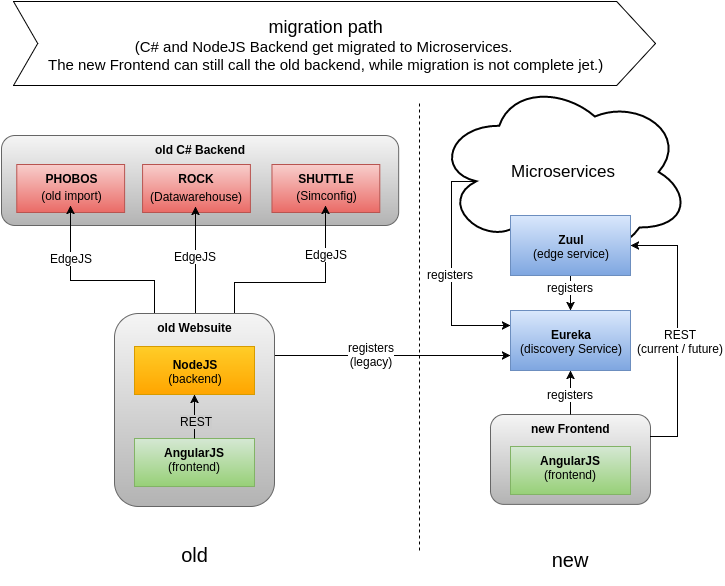
\includegraphics[width=1\textwidth]{res/Websuite_migration}
	\caption{Websuite migration path}
	\label{fig:websuite-migration}
\end{figure}

The old JavaScript stack, containing of an AngularJS front-end and an NodeJS back-end with connection to the C$\sharp$ code over EdgeJS was replaced. The NodeJS components were migrated to several micro-services and the front-end was converted to a WebUI micro-service that consists of an AngularJS front-end with a thin layer of NodeJS to host the application.\\
The process of migrating to the new structure is complete and the old monolithic Websuite is not used anymore.



\section{Tooling}
To effectively develop a front-end application, certain talks have to be done, to make the process convenient in development and usable in production. The following topics have to be considered.


\subsection{Dependency management}
Almost every application depends on third-party components. Manually managing dependencies is an error prone tasks and checking them into the version control system clutters its history.\\
This is why the WebUI uses the \textit{Node Package Manager} (NPM) and Bower. NPM is responsible for managing NodeJS dependencies that are used for tooling and serving the Anguular app. Bower takes care of the front-end libraries. Both tools depend on a JSON file that lists the needed dependencies, as well as their required version. This guarantees that any deployment of the app uses the correct version of any used library.

\subsection{Task Runner}
A task runner allows to run various tasks that are used during the development process. The WebUI uses Gulp, which is responsible for executing the following tasks.

\subsubsection{Live reload} Restarts the application and reloads the website inside the browser, once the source code has changed. It is only used for development.

\subsubsection{Browser sync} Synchronizes the active state of all open browser windows. This helps testing cross-browser compatibility in development.

\subsubsection{Combining files} Combines all files of a type (e.g. .js, .html or .css) to one file. This reduces the amount of connections needed to serve the page in production and therefore improves load time.

\subsubsection{Uglifying} Renames variables and functions to single character names to reduce the size of the served files in production.

\subsubsection{minifying} Removes spaces and line-breaks, to further reduce the file size in production.

\subsubsection{Compiling SCSS}
Compiles the SCSS styles to CSS. For further information see section \ref{sec:styling}.


\subsection{Initial Configuration}
\label{sec:initial_config}
The tasks above need to be configured, to match the development work-flow and the used file structure. This initial configuration was created with a tool called \textit{generator-gulp-angular} and modified to match the actual need for the WebUI. Additionally the generator created the file structure for the new WebUI.



\section{Migrating the application}
While it was possible to simply strip out old parts and reuse the old Websuite's code-base, this was not done. Instead, a completely new structure with tested tooling was created, using the previously mentioned generator-gulp-angular (see section \ref{sec:initial_config}). This guaranteed that no old code was left inside the application, which could cause problems in the future.\\


\subsection{Styling}
\label{sec:styling}
The styling of the old application was discarded, because it contained of many lines of self-written CSS that had no unified look and was not responsive for the most part. Instead the layout is now done, using bootstrap with minimal adjustments at certain points.\\
To prevent visual side effects in other components, every html template is wrapped in a div, with its components name as the id. The CSS file for every component is only applied to children of this id.\\
To further improve the simplicity of the styling \textit{Sassy CSS} (SCSS) was used to write styles. SCSS is a CSS preprocessor that is compiled to CSS and adds features like variables, reusable components, loops and nesting.\\
The fact that it uses CSS syntax, allows a smooth transition, because the developer can use it like normal CSS and make use of the additional features when ever he desires.


\subsection{Components}
The following components were migrated.

\subsubsection{Import}
As part of the the migration, the two imports data and model were migrated to one code-base. This was done, by creating an import directive, that can be parameterized upon usage. The merge eliminated duplicate code and resolved already existing variation in the behavior of the imports.\\
The process that is shown in figure \ref{fig:import} shows the way, the import interacts with the back-end. Once the user selects one or more files, the WebUI generates one input form for every file. An exception is the \textit{bulk upload}. If this option is enabled, one form is generated for all files. The forms are validated while the user inputs data, to prevent mistakes as early as possible.\\
Once the user starts the upload, the files are successively send to the \textit{File Service}. During that process the upload progress is shown. When the file have been uploaded, the WebUI triggers the long-polling. This is done independent of the the import page and the current state is therefore visible from any page. Also, the user may leave the page and come back later to check, if the processing was successful.\\
To trigger the long-polling, the WebUI sends an GET request to the \textit{Metadata Service} and and \enquote{init} as the current state. The server responds with the current state and the WebUI sends a new request using the received state. From now on, the Metadata Service answers, as soon as the stat has changed and the front-end immediately requests again. This process is repeated until the import is either successful or failed.
\begin{figure}[H]
	\centering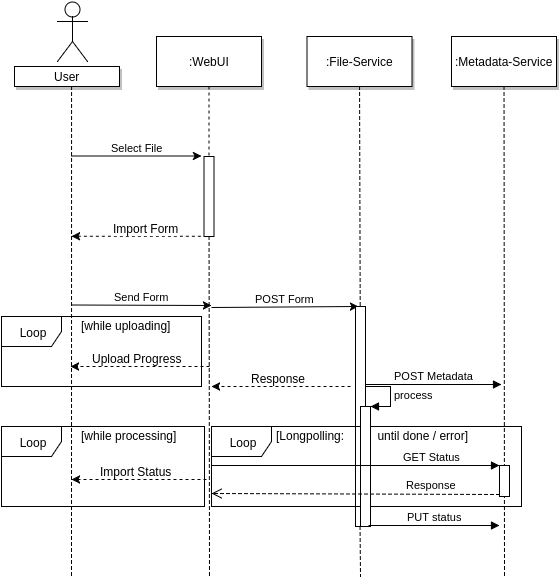
\includegraphics[width=.75\textwidth]{res/Import}
	\caption{Import}
	\label{fig:import}
\end{figure}


\subsubsection{Data View}


\subsubsection{Scenario}
\begin{figure}[H]
	\centering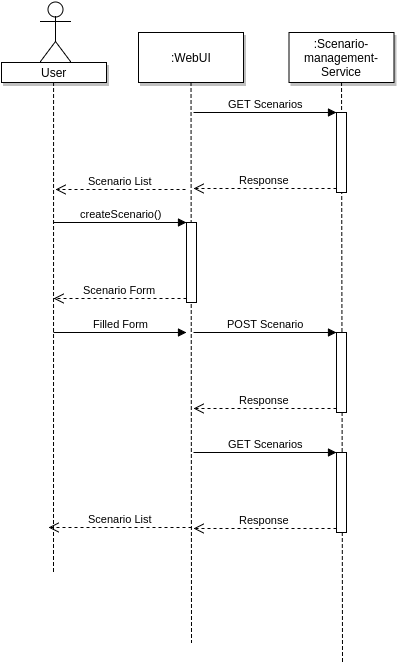
\includegraphics[width=.65\textwidth]{res/Scenario}
	\caption{Scenario}
	\label{fig:scenario}
\end{figure}


\subsubsection{Mapping}
\begin{figure}[H]
	\centering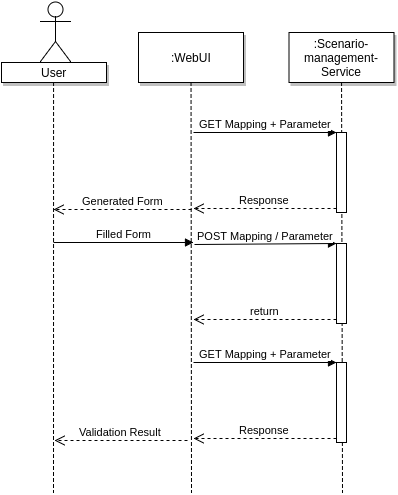
\includegraphics[width=.65\textwidth]{res/Mapping}
	\caption{Mapping}
	\label{fig:mapping}
\end{figure}




\section{Error Handling}
% Display of error messages to the user
% Dashboard to show service availability
